\section{Méthodes possibles pour la virtualisation légère}
\label{section:emulation}

Il existe actuellement deux méthodes permettant de faire de la virtualisation
légère. La première est une émulation par limitation ou dégradation également
appelée virtualisation standard et la seconde est une émulation par
interception.

\begin{figure}[H]
  \centering 
  \begin{subfigure}{0.3\textwidth}
    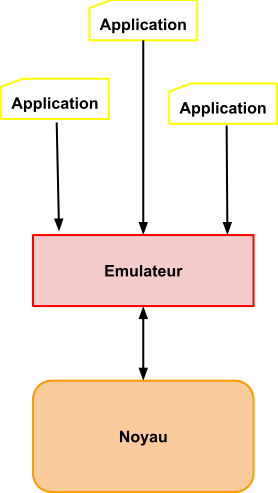
\includegraphics[scale=0.35]{Pictures/png/Virtualisation_limitation}
  \end{subfigure}
  \begin{subfigure}{0.3\textwidth}
    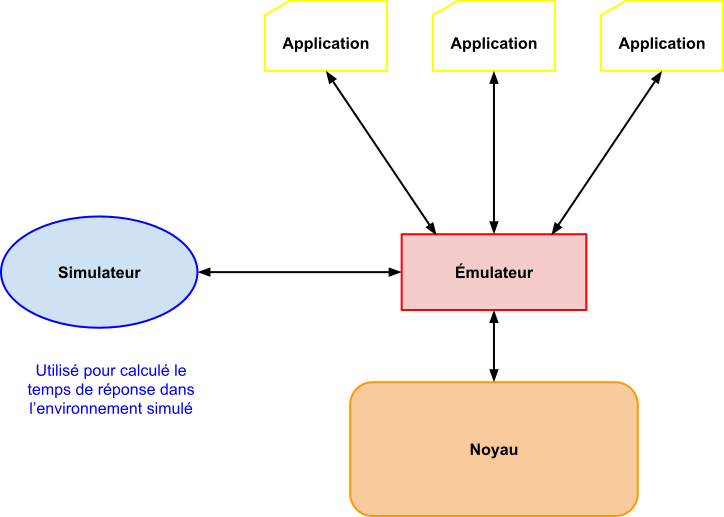
\includegraphics[scale=0.3]{Pictures/png/Virtualisation_interception}
  \end{subfigure}
  \caption{Virtualisation par limitation (à gauche) et par interception (à
    droite)}
  \label{TYPE_VIRTUALISATION}
\end{figure}

\subsection{Virtualisation standard}
\label{section:limitation}
%% \begin{itemize}
%% \item principe: limiter l'accès aux ressources par exemple (cgroup, netstat, cpuburner), temps d'un SEB (bench avec netlink, limiter (cap))
%% \item avantage plus simple
%% \item désavantages: host>>target, modèle à vérifier, contrôle expérimental fin
%% \end{itemize}

Avec cette première méthode, illustrée Fig.\ref{TYPE_VIRTUALISATION}, on place la couche d'émulation au-dessus de la
plateforme réelle (comme un hyperviseur pour une VM). De fait, la puissance de
l'émulateur dépend de la puissance de la machine hôte et ne peux donc pas
dépasser les capacités de cette dernière. De plus, en choisissant de placer
l'émulation comme une surcouche, cela permet de limiter l'accès aux ressources
pour les applications. En effet, elles ne pourront pas passer la couche
d'émulation pour accéder aux ressources localisées sur la machine hôte. Les
requêtes des applications distribuées seront arrêtées par l'émulateur. C'est lui
qui s'occupera de récupérer les ressources demandées par les applications. Il
existe différents outils permettant de mettre en place cette virtualisation, on
trouve notamment \textbf{cgroup}, \textbf{netstat} et \textbf{cpuburner}.  L'émulation par limitation a l'avantage d'être simple à mettre en \oe uvre puisque
l'on se base sur la machine hôte. Néanmoins elle est assez contraignante du fait
qu'on ne puisse pas émuler des architectures plus performantes que l'hôte. De
plus {\color{red} \textit{à écrire deux derniers points négatifs à éclaircir}}.

\subsection{Émulation par interception}
%% principe: interception des actions et médiation (pas juste interception et rejeu). Intercepter des symboles pour en changer l'effet

Dans le cas de l'émulation par interception, illustrée
Fig.\ref{TYPE_VIRTUALISATION}, pour mettre en place un environnement distribué
émulé sur lequel les applications penseront s'exécuter, deux outils vont être
utilisés; un simulateur pour virtualiser l'environnement d'exécution, et un
émulateur qui va attraper toutes les communications de l'application avec l'hôte
et qui les transmettra ensuite au simulateur.
%%  Les calculs de l'application seront effectués sur la machine hôte
%% mais c'est le simulateur qui calculera le temps de réponse à l'application. Pour
%% cela il fera un rapport entre le temps d'exécution du calcul sur la machine hôte
%% (fourni par l'émulateur qui le mesure lors de l'exécution du calcul), la
%% puissance de l'hôte et celle des machines de l'environnement que l'on simule. Le
%% temps de l'application sera donc celui du simulateur et non le temps réel. En
%% effet, \textit{si on se base sur l'horologe de la machine hôte pour gérer le
%%   temps de l'application, il faudra pour chaque calcul trouver la différence de
%%   temps entre l'exécution sur l'hôte et celle sur la plateforme émulée pour
%%   décaler l'horloge de l'application et maintenir la virtualisation de
%%   l'environnement distribué. Avec cette solution on ne se contente pas de faire
%%   de l'interception d'action et du rejeu par l'émulateur comme c'est le cas avec
%%   l'émulation par limitation. On va intercepter les actions des applications et
%%   les modifier avant de les laisser s'exécuter sur la plateforme réelle sous le
%%   contrôle de l'émulateur pour maintenir la vision d'un environnement distribuée
%%   pour l'application. Ce mécanisme s'appelle la médiation.}

 Une application distribuée peut vouloir communiquer avec l'hôte soit pour
 effectuer de simples calculs {\color{red}\textbf{TODO}}(SEB), soit pour effectuer des requêtes de
 connexion ou de communication avec d'autres applications sur le réseau. Quand
 l'émulateur intercepte une communication venant d'un des processus d'une
 application, il modifie les caractéristiques de cette dernière pour qu'elle
 puisse s'exécuter sur la machine hôte. Quand cette dernière renvoie une réponse
 à l'application, elle est également interceptée par l'émulateur pour que
 l'application ne voit pas le changement d'architecture. En même temps, il
 envoie au simulateur le temps d'exécution de l'action sur la machine hôte pour
 qu'il puisse calculer ce temps sur la machine simulée, en faisant un rapport
 entre les performances des deux machines. Les délais calculés par le simulateur
 sont soit des temps de calculs soit des temps de connexion ou de
 communication. Lorsque le simulateur a terminé le calcul du temps de réponse,
 il le transmet à l'émulateur qui l'envoie à l'application en plus du résultat
 du calcul demandé pour mettre à jour son horloge. Ainsi, les calculs sont
 réellement exécutés sur la machine, les communications réellement émises sur le
 réseau géré par le simulateur et c'est le temps de réponse qu'il fourni qui va
 influencer l'horloge de l'application. Finalement, les applications ne
 communiquent plus directement entre elles.

 \begin{figure}
   \centering
   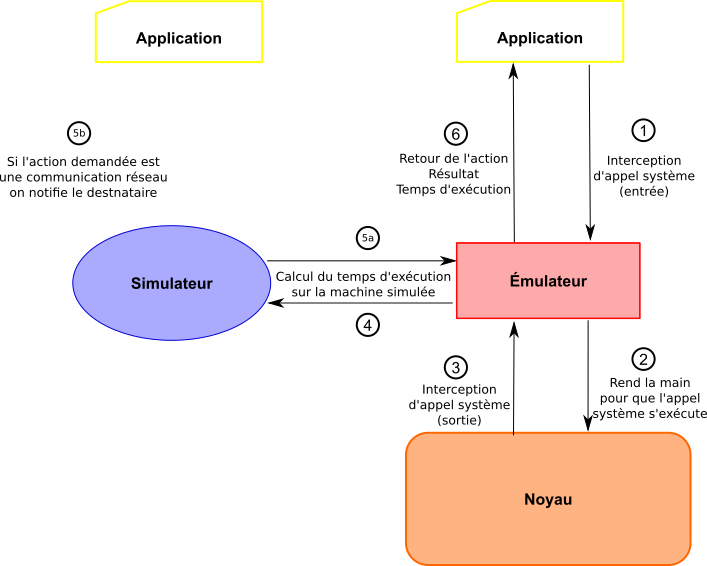
\includegraphics[scale=0.5]{Pictures/png/Emulation_fonctionnement}
   \caption{Fonctionnement de l'émulation par interception}
   \label{INTERCEPTION}
 \end{figure}
 
Pour intercepter ces actions, il faut d'abord choisir à quel niveau se placer.
%% : code source ou binaire. Mais il faut également choisir sur quel
%% type de symbole (appel système, appel de fonction...), utilisé par l'application
%% pour exécuter ses actions, et avec quel outil l'émulateur fera des modifications permettant de maintenir la vision d'un environnement distribué. Par la suite on a ppelera médiation l'ensemble de ces modifications.
%%     qui suit l'interception et avec quel
%% outil.
 En effet, une application peut communiquer avec le noyau via différentes
 abstractions. Elle peut soit utiliser les fonctions d'interaction directe avec
 le noyau que sont les appels systèmes, soit utiliser les différentes
 abstractions fournies par le système d'exploitation: bibliothèques (fonctions
 de la libc par exemple) ou les fonctions POSIX dans le cas d'un système UNIX.

\begin{figure}[H]
 \centering
 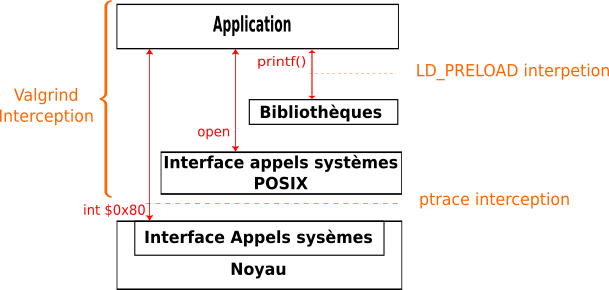
\includegraphics[scale=0.75]{Pictures/png/Communication_application_noyau_v3.png}
 \caption{Communications possibles entre le noyau et une application}
 \label{AS_Communication}
\end{figure}

Nous allons donc voir comment on peut intercepter et modifier des actions au
niveau de l'application (fichier source puis binaire), des appels systèmes et
des appels de fonctions. Par la suite nous appelerons médiation l'ensemble des
modifications effectuées par l'émulateur sur les actions interceptées.
%% {\color{red} L'interception des actions d'une application peut se faire à deux niveaux: sur le fichier source et sur le binaire. La médiation qui suit l'interception des actions peut également se faire sur différent type de symboles: les appels de focntions et les appels systèmes.  \textit{mettre partie ce qu'on intercepte pourquoi et le schéma}}

\subsubsection{Action sur le fichier source}
%% reimplem SMPI (trop spé) ,source to source/ pass LLVM( gcc+libc=consanguin) 
%% , Coccinelle

\subsubsection{Action sur le binaire}
%%Valgrind (perf pourrie)
Pour agir sur le binaire d'une application, c'est l'outil d'instrumentation
d'analyse dynamique Valgrind \citep{Valgrind, Valgrindweb} que nous allons étudier. À l'origine, il est utilisé
pour le débuguage mémoire, puis il a évolué pour devenir l'instrument de base à
la création d'outils d'analyse dynamique de code, tels que la mise en évidence
de fuites mémoires ou le profilage\footnote{Méthode visant à analyser le code
  d'une application pour connaître la liste des fonctions appelées et le temps
  passé dans chacune d'elles}. Valgrind fonctionne à la manière d'une machine
virtuelle faisant de la compilation à volée\footnote{Technique basée sur la
  compilation de byte-code et la compilation dynamique. Elle vise à améliorer la
  performance de systèmes bytecode-compilés par la traduction de bytecode en
  code machine natif au moment de l'exécution}. Ainsi, ce n'est pas le code
initial du programme qu'il envoie au processeur de la machine hôte. Il traduit
d'abord le code dans une forme simple appelée ``Représentation Intermédiaire''. Ensuite, un des outils d'analyse dynamique de Valgrind peut être
utilisé pour faire des transformations sur cette ``Représentation
Intermédiaire''. Pour finir, Valgrind traduit la ``Représentation
Intermédiaire'' en langage machine et c'est ce code que le processeur de la
machine hôte va exécuter. De plus, grâce à la compilation dynamique, Valgrind
peut recompiler certaines parties du code d'un programme durant son exécution et
donc ajouter de nouvelles fonctions au code de l'application.

Dans notre cas, on peut utiliser Valgrind pour mesurer le temps passé à faire un
calcul. Ce dernier étant ensuite envoyé au simulateur pour calculer le temps de
réponse dans l'environnement simulé nécessaire à l'émulateur. On pourrait
également l'utiliser pour réécrire à la volée le code des fonctions que
l'émulateur doit modifier pour maintenir la virtualisation. Pour faire cela, il
faut créer un ``wrapper'' pour chaque fonction qui nous intéresse. Un wrapper
Valgrind est une fonction de type identique à celle que l'on souhaite
intercepter, mais ayant un nom différent (généré par les \texttt{macro} de
Valgrind) pour la différencier de l'originale. Pour générer le nom du wrapper
avec les \texttt{macro} de Valgrind on doit préciser la bibliothèque qui
contient la fonction originale.%% et
%% utiliser un Z-encodage\footnote{ Permet de rendre des caractères valides pour
%%   des noms de fonction en C, Z est le caractère d'échappement pour. Par exemple
%%   : Za pour *, Zp pour +, Zc = :,
%%   ... \\ \url{http://valgrind.org/docs/manual/manual-core-adv.html}}. Cette
%% opération est lourde et complexe. De plus, elle nécessite de connaître le nom de
%% la bibliothèque qui contient la fonction qui nous intéresse
Cela implique donc de connaître pour chaque fonction à intecepter le nom de la
librairie qui l'implémente. Cette solution est donc assez contraignante et ses
performances sont assez médiocres d'après l'étude faite par M. Guthmuller lors
de son stage \citep{MARION:Interception}: facteur de 7.5 pour le temps
d'exécution d'une application avec cet outil. Cette perte de performance est due
à la compilation faite en deux phases ainsi qu'au temps nécessaire aux outils de
Valgrind pour modifier ou rajouter du code à l'existant. Cela pourrait être
acceptable, si Valgrind faisait de la traduction dynamique lors de la seconde
phase de sa compilation, nous permettant ainsi d'avoir du code exécutable sur un
autre type de processeur que celui de l'hôte, mais ce n'est pas le cas.

\subsubsection{Médiation des Appels Système}
%% pourquoi: read/write, comm reseau 

En regardant la Fig.\ref{AS_Communication} et les différents niveaux
d'abstractions, le moyen le plus simple pour attraper les actions de
l'application en gérant un minimum de choses est d'intercepter directement les
appels systèmes.  Ces derniers sont constitués de deux parties; la première,
l'entrée, initialise l'appel via les registres de l'application qui contiennent
les arguments de l'appel puis donne la main au noyau. La seconde, la sortie,
inscrit la valeur de retour de l'appel système dans le registre de retour de
l'application, les registres d'arguments contenant toujours les valeurs reçues à
l'entrée de l'appel système, et rend la main à l'application. \textit{Nous
  devons donc bloquer l'application à chaque interception d'une deux parties de
  l'appel système. Nous permettant ainsi de récupérer et modifier les
  informations permettant de maintenir l'environnement simulé avant de lui
  rendre la main, pour pouvoir entrer ou sortir de l'appel système.}

 Dans cette section, nous allons présenter les outils existants qui permettent
 de faire cela.
 
 \paragraph{L'appel système ptrace}\citep{AS:Interception, MARION:Interception}
 , dont la Fig.\ref{PTRACE_FONCTIONNEMENT} illustre le fonctionnement, permet de
 tracer tous les événement désirés d'un processus. Il peut également lire et
 écrire directement dans l'espace d'adressage de ce dernier, à n'importe quel
 moment ou lorsque un événement particulier se produit. De cette façon on peut
 contrôler l'exécution d'un processus. C'est un appel système dont chaque action
 à effectuer est passée sous forme de requêtes en paramètre de l'appel système.

Pour pouvoir contrôler un processus via \texttt{ptrace}, on va créer deux
processus parents via un \texttt{fork}(); un processus appelé ``processus
espionné'' qui exécutera l'application et qu'on souhaite contrôler, et un autre
qui contrôlera le processus espionné, appelé ``processus espion''. Le processus
espionné indiquera au processus espion qu'il souhaite être contrôlé via un appel
système \texttt{ptrace} et une requête \texttt{PTRACE\_TRACEME} puis il
exécutera l'application via un \texttt{exec}(). À la réception de cet appel, le
processus espion notifiera son attachement au processus espionné via un autre
appel à \texttt{ptrace} et une requête \texttt{PTRACE\_ATTACH}. Il indiquera
également sur quelles actions du processus espionné il veut être notifié (chaque
instruction, signal, sémaphore...), définissant ainsi les actions bloquantes
pour le processus espionné. Dans notre cas, ce seront les appels systèmes que
l'on considérera comme points d'arrêts (requête
\texttt{PTRACE\_SYSCALL)}. Ainsi, le processus espion sera donc appelé deux
fois: à l'entrée et à la sortie de l'appel système.

Quand un des processus de l'application voudra faire un appel système, il sera
bloqué avant de l'exécuter et le processus espion qui lui est associé sera
notifié via un appel système \texttt{ptrace}. Ce dernier fera alors les
modifications nécessaires dans les registres du processus espionné pour
conserver la virtualisation de l'environnement. Pour cela il pourra utiliser les
requêtes \texttt{PEEK\_DATA} et \texttt{POKE\_DATA} passées en argument de
l'appel système {\color{red} (à éclaircir)\textbf{ou modifier directement le
    contenu du /proc/id/mem}}. Puis, il rendra la main au processus espionné
pour que l'appel système puisse avoir lieu.%% Au retour de
%% l'appel système le processus espionné sera de nouveau stoppé et un \texttt{ptrace} sera
%% envoyé au processus espion qui remodifiera les informations nécessaires. Puis il
%% rendra la main au processus espionné bloqué qui sortira de son appel système
%% avec un résultat exécuté sur la machine hôte et un temps d'exécution et une
%% horloge fournie par le simulateur.
 Le même fonctionnement est utilisé pour le retour de l'appel
 système. \textit{Le processus espion change simplement le temps d'exécution de
   l'appel système et l'horloge de l'application en utilisant ceux calculés par
   le simulateur.}  Quand un processus espion a fini un suivi, il peut envoyer
 deux types de requêtes au processus espionné: \texttt{PTRACE\_KILL} qui termine
 le processus espionné ou \texttt{PTRACE\_DETACH} qui le laisse continuer son
 exécution.

\begin{figure}
   \centering
   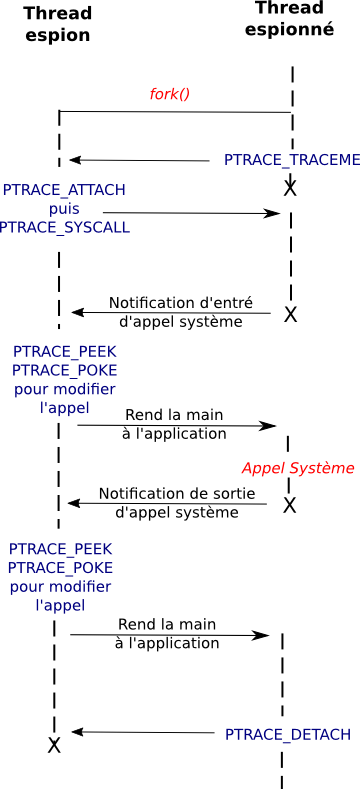
\includegraphics[scale=0.5]{Pictures/png/ptrace_fonctionnement}
   \caption{Attachement d'un processus et contrôle via un espion}
   \label{PTRACE_FONCTIONNEMENT}
 \end{figure}
 
Néanmoins, pour contrôler un processus, \texttt{ptrace} fait de nombreux
changements de contexte pour pouvoir intercepter et gérer les événements, or
cela coûte plusieurs centaines de cycle CPU. \textit{De plus, il supporte mal
  les processus utilisant du multithreading, et ne fait pas parti de la norme
  POSIX. Ainsi il peut ne pas être disponible sur certaines architectures et son
  exécution peut varier d'une machine à une autre.}

\paragraph{Uprobes}\citep{AS:Interception, MARION:Interception}
%% Non module noyau

%% pour \textit{user-space probes}, quant à lui permet d'insérer dynamiquement des
%% points d'arrêts à n'importe quel endroit dans le code d'une application, dans
%% notre cas les appels systèmes. Pour chaque point d'arrêt, l’utilisateur fournit
%% un handler particulier à exécuter avant ou après l’instruction marquée. Uprobes
%% étant un outil s'exécutant dans le noyau, les handlers doivent être placé dans
%% un module. Pour chaque point d'arrêt géré par Uprobes, le module noyau contient
%% le handler à exécuter, ainsi que le processus et l'adresse virtuelle du point
%% d'arrêt. Lorsqu'un point d'arrêt est atteint Uprobes prend la main et exécute le
%% bon handler. Pour savoir qu'un point d'arrêt a été touché, Uprobes utilise
%% Utrace, équivalent de ptrace en mode noyau. Ce dernier permet d'éviter les
%% nombreux changements de contexte et est capable de gérer le
%% multithreading. Utrace peut également être utilisé dans le module gérant un
%% point d'arrêt pour récupérer des informations sur l'application et les données
%% qu'elle utilise.

%% Les deux avantages de cette solution sont qu'elle est rapide et qu'elle a accès
%% à toutes les ressources sans aucune restriction. Mais ce dernier point
%% représente aussi son plus gros défaut de par sa dangerosité. De plus, dans notre
%% cas il ne semble pas judicieux de faire de la programmation noyau via un
%% module dont l'utilisateur devra également gérer le bon chargement.

pour \textit{user-space probes}, quant à lui est une API noyau permettant
d'insérer dynamiquement des points d'arrêts à n'importe quel endroit dans le
code d'une application, dans notre cas les appels systèmes, et à n'importe quel
moment de son exécution.

Il existe deux versions de Uprobes la première est basée sur les ``trace
hook\footnote{\url{http://fr.wikipedia.org/wiki/Hook\_\%28informatique\%29}}''\textbf{{\color{red}citation}}. Cette
solution ne sera pas développée ici car elle est très peu utilisée
\textbf{{\color{red} à vérifier}}.

La seconde, la plus connue, se base sur Utrace, équivalent de \texttt{ptrace} en
mode noyau. Ce dernier permet d'éviter les nombreux changements de contexte, qui
dégradent les performances, et est capable de gérer le multithreading. Dans
cette version, l'utilisateur fournit pour chaque point d'arrêt un handler
particulier à exécuter avant ou après l’instruction marquée. Uprobes étant un
outil s'exécutant dans le noyau, les handlers doivent être placés dans un module
noyau. Ce dernier contient pour chaque point d'arrêt géré par Uprobes le handler
à exécuter, ainsi que le pid du processus concerné et l'adresse virtuelle du
point d'arrêt. Pour gérer un point d'arrêt Uprobes utilise trois structures de
données \textit{i)} \texttt{uprobe\_process} (une par processus controlé),
\textit{ii)} \texttt{uprobe\_task} (autant que le processus contrôlé a de
thread), \textit{iii)} \texttt{uprobe\_kimg} (une pour chaque point d'arrêt
affectant un procesus). Chaque structure \texttt{uprobe\_task} et
\texttt{uprobe\_kimg} sont propres à une structure \texttt{uprobe\_process}. La
fonction \texttt{init}() du module va poser les points d'arrêt et la fonction
\texttt{exit}() les enlevera. Pour cela on utilise respectivement la fonction
\texttt{register\_uprobe} et \texttt{unregister\_uprobe}. Ces deux fonctions ont
pour argument le pid du processus à contrôler, l'adresse virtuelle du point
d'arrêt dans le code et le handler à exécuter quand le point d'arrêt est
atteint. La fonction \texttt{register\_uprobes} va trouver le processus passé en
paramètres en parcourant la liste des structures \texttt{uprobes\_process} ou la
crééra si cette dernière n'existe pas. Ensuite, elle crée la structure
\texttt{uprobe\_kimg}, puis fait appel à Utrace pour bloquer l'application, le
temps de placer le point d'arrêt dans le code de celle-ci. Pour cela, on va
placer avant l'instruction sondée un appel au module contenant le handler à
invoquer, puis on rend la main à l'application en utilisant de nouveau
Utrace. \texttt{unregister\_uprobe} fait de même mais supprime la structure
\texttt{uprobe\_kimg} passée en paramètre au lieu de l'ajouter. De plus, s'il
s'agit de la dernière structure de ce type pour un processus contrôlé, il
supprimera alors la structure \texttt{uprobe\_process} et toutes les
\texttt{uprobe\_task} associées.

Lorsqu'un point d'arrêt est atteint Uprobes prend la main et exécute le bon
handler. Pour savoir qu'un point d'arrêt a été touché, Uprobes utilise de
nouveau Utrace, ce dernier envoyant un signal à Uprobes à chaque fois que le
processus qu'il contrôle atteint un point d'arrêt.

Utrace envoie également un signal à Uprobes quand un des processus contrôlé fait
un appel à \texttt{fork}()/\texttt{clone}(), \texttt{exec}(), \texttt{exit}()
pour que ce dernier créé ou supprime les structures uprobe\_process
concernées. Utrace peut également être utilisé dans le handler gérant un point
d'arrêt pour récupérer des informations sur l'application et les données qu'elle
utilise. De plus, un handler peut également ajouter ou enlever des points
d'arrêts.

Les deux avantages de cette solution sont qu'elle est rapide et qu'elle a accès
à toutes les ressources sans aucune restriction. Mais ce dernier point
représente aussi son plus gros défaut de par sa dangerosité. De plus, dans notre
cas il ne semble pas judicieux de faire de la programmation noyau via un module
dont l'utilisateur devra également gérer le bon chargement.

\paragraph{Seccomp/BPF:}
%% Read only

Seccomp \citep{seccompbpf} est un appel système qui permet d'isoler un processus
en lui donnant le droit d'appeler et d'exécuter qu'un certain nombre d'appels
systèmes: \textit{read}, \textit{write}, \textit{exit} et \textit{sigreturn}. Si
le processus fait un autre appel système, il sera arrêté avec un signal
\texttt{SIGKILL}. Comme cela est assez contraignant, le nombre d'applications
que l'on peut utiliser avec seccomp est donc très limité. Pour plus de
flexibilité, on peut utiliser une extension de cet appel système appelée
seccomp/BPF, pour \textit{seccomp BSD Packet Filter}, permettant de définir dans
un programme BPF \citep{BPF_mccanne1993bsd} les appels systèmes autorisés à
s'exécuter, en plus de ceux cités précédemment. Cette dernière fonctionne sur le
même principe que le filtrage de paquet réseau où on établit une suite de
règles. Pour pouvoir s'exécuter, un appel système doit pouvoir passer à travers
toutes les règles. Dans le cas où les appels systèmes \texttt{fork}() ou
\texttt{clone}() peuvent s'exécuter, l'arborescence de filtres est transmise aux
enfants, de même que pour les processus faisant des appels \texttt{execve}()
quand ils sont autorisés. Les règles des filtres BPF portent sur le type de
l'appel système et/ou ses arguments. Ainsi, à chaque entrée ou sortie d'un appel
système, ne faisant pas partie des quatre autorisés par seccomp, l'extension
utilisant BPF est appelée. Elle reçoit en entrée le numéro de l'appel système,
ses arguments et le pointeur de l'instruction concernée. En fonction des règles,
elle laisse l'appel système s'exécuter ou pas.  De plus, seccomp/BPF possède une
option qui lui permet de générer un appel système \texttt{ptrace}(). Cela permet
au processus espion, s'il existe, de ne plus attendre sur chaque appel système
du processus espionné, mais uniquement sur les appels systèmes qu'il souhaite
intercepter.

Néanmoins, l'appel système seccomp et son extension seccomp/BPF ne sont
disponibles que si le noyau est configuré avec l'option \texttt{CONFIG\_SECCOMP}
pour la première et \texttt{CONFIG\_SECCOMP\_FILTER} pour la deuxième. Pour
pouvoir créer des filtres, il faut également avoir des droits particuliers,
notamment l'exécution de certaines commandes root. Ainsi, l'utilisation de cet
appel système et de son extension demande une certaine configuration noyau et
des privilèges pour les utilisateurs, ce qui n'est pas très conseillé.

De plus, si on l'utilise sans l'option d'appel à \texttt{ptrace} on ne peut que
lire le contenu de l'appel système et pas le modifier. On ne peut donc pas faire
de médiation avec cet outil sans faire appel à \texttt{ptrace}. Néanmoins,
l'utilisation de seccomp/BPF avec \texttt{ptrace} permet de réduire
signifiquativement le nombre d'événement sur lequel attendra le processus
espion.
\newline
Malgré ses défauts, l'appel système \texttt{ptrace} semble être le meilleur
outil pour faire ce type d'interception. Néanmoins, il a été montré dans un
précédent stage \citep{MARION:Interception} qu'il est inefficace voire inutile
en ce qui concerne tous les appels systèmes temporels qu'une application
souhaiterait exécuter (\texttt{time}(), \texttt{clock\_gettime}(),
\texttt{gettimeofday}()) car le noyau ne les exécute pas. Cela est du à
l'existence de la bibliothèque \textit{Virtual Dynamic Shared Object}
(VDSO). Cette dernière vise à minimiser les coûts dûs aux deux changements de
contexte effectués lors de l'exécution d'un appel système. VDSO va retrouver
l'heure \textit{{\color{red}dans le contexte noyau}} lisible par tous les
processus sans changer de mode. Il est possible de désactiver cette bibliothèque
lors du boot mais cela réduit les performances (plus de changements de contexte)
et oblige l'utilisateur à modifier les paramètres de son noyau. On peut donc
dire que cette solution d'interception n'est donc pas complète.

%%avec \textbf{ptrace} ne sont pas possibles, d'où l'alliance
%%   avec LD\_PRELOAD} Par exemple lors d'un gettimeofday l'appel système n'est pas
%% lancé on répond directement au niveau de la bibliothèque ainsi on n'arrive même
%% pas au niveau de l'appel système, donc ptrace ne fait rien.  Problème
%% portabilité {\color{red} \textbf{gérer cette transition}}

\subsubsection{Médiation directe des appels de fonctions}
%%pourquoi: pthread, temps

Puisque l'interception des actions d'une application au plus bas niveau ne
suffit pas, on peut penser qu'une bonne solution est d'intercepter les actions
de l'application au plus haut niveau que sont les bibliothèques. Pour cela nous
allons étudier deux approches basées sur l'éditeur de liens dynamiques de Linux
qui permet d'insérer du code dans l'exécution d'un programme.

\paragraph{LD\_PRELOAD:}
\label{paragraphe:LDPreload}
%pas suid

L'utilisation de la variable d'environnement \texttt{LD\_PRELOAD}
\citep{LDPreload}, contenant une liste de bibliothèques partagées, va nous
permettre d'intercepter les appels aux fonctions qui nous intéressent et d'en
modifier le comportement. Cette variable est utilisée à chaque lancement d'un
programme par l'éditeur de liens pour charger les bibliothèqes partagées qui
doivent être chargées avant toute autre bibliothèque (même celles utilisées par
le programme). Ainsi, si une fonction est définie dans plusieurs bibliothèques
différentes, celle utilisée par le programme sera celle qui est contenue dans la
bibliothèque partagée apparaîssant en premier dans la liste des bibliothèques
préchargées. Ce ne sera pas \textit{nécessairement} celle de la bibliothèque
attendue par le programme. Par exemple, on créé une bibliothèque partagée qui
implémente une fonction open() de même prototype que la fonction open() de la
libc et on place cette bibliothèque dans la variable \texttt{LD\_PRELOAD}. Quand
on exécute un programme faisant un appel à open(), l'éditeur de lien va d'abord
charger les bibliothèques contenues dans la variable d'environnement
\texttt{LD\_PRELOAD} puis la libc, la nouvelle bibliothèque apparaîtra donc
avant la libc dans la liste des bibliothèques préchargées. Ainsi, c'est la
nouvelle fonction open() qui sera exécutée par le programme et non
l'originale. De cette façon, on peut intercepter n'importe quelle fonction.

Dans notre cas, on va donc créer notre propre bibliothèque de fonctions. Pour
chaque fonction susceptible d'être utilisée par l'application, on crééra une
fonction de même nom et de même type dans notre bibliothèque. Chacune de nos
fonctions contiendra alors toutes les modifications nécessaires pour maintenir
notre environnement simulé suivi d'un appel à la fonction initiale. On rappelle
que dans notre cas, on souhaite juste intercepter l'appel et pas l'empêcher.
%%Pour faire
%% appel à la fonction initiale on ne peut pas simplement l'appeler par son nom
%% puisque ce serait notre nouvelle fonction qui serait appelée. On va donc utiliser
%% dans notre nouvelle fonction les fonctions de la famille dlopen, notamment
%% dlopen et dlsym. La première permet de charger une bibliothèque dynamique dont
%% le nom est passé en paramètre et de récupérer un
%% ``handle''\footnote{http://pubs.opengroup.org/onlinepubs/009695399/functions/dlopen.html
%%   \\ A successful dlopen() shall return a handle which the caller may use on
%%   subsequent calls to dlsym() and dlclose(). The value of this handle should not
%%   be interpreted in any way by the caller.} utilisé par dlsym pour trouver
%% l'adresse de la fonction originale qui nous intéresse en mémoire, nous
%% permettant ainsi d'y faire appel.
Notre nouvelle bibliothèque sera préchargée avant les autres en la plaçant dans
la variable \texttt{LD\_PRELOAD}, ainsi nos fonctions passeront avant les
fonctions des bibliothèques usuelles.

Néanmoins, si l'application fait un appel système directement sans passer par la
couche \textit{Bibliothèques} (Fig.~\ref{AS_Communication}) notre mécanisme
d'interception est contourné. \textit{En effet on ne peut surcharger que des
  fonctions définies dans bibliothèques avec cette solution, pas les appels
  systèmes directement.} De même, si on oublie de réécrire une fonction d'une
des bibliothèques utilisée par l'application. Cette solution n'est donc pas
suffisante pour le modèle d'interception que nous souhaitons avoir.

Cependant, on peut voir que \texttt{LD\_PRELOAD} résout les lacunes de
\texttt{ptrace} concernant les fonctions de temps et le multithreading. À
l'inverse, puisque \texttt{ptrace} permet d'intercepter les appels systèmes que
le modèle d'interception avec \texttt{LD\_PRELOAD} ne permet pas de gérer, on
peut dire que \texttt{ptrace} résout les problèmes de \texttt{LD\_PRELOAD}. Une
solution choisie lors d'un précédent stage est donc d'allier les deux. On
surchargera les fonctions temporelles dans notre bibliothèque préchargée avec
\texttt{LD\_PRELOAD} pour pallier les lacunes temporelles de
\texttt{ptrace}. \textit{Et ce dernier s'occupera de toutes les autres
  fonctions}, ainsi on est certain de n'oublier aucune fonction.

\paragraph{Got injection:}
%% plus dur que nécessaire

\begin{table}[H]
\begin{tabular}{c|c|c|c|c|}
\cline{2-5} & Source to Source & \begin{tabular}[c]{@{}c@{}}Réimpplémentation
  \\ SMPI\end{tabular} & Coccinelle & Valgrind \\ \hline
  \multicolumn{1}{|c|}{\begin{tabular}[c]{@{}c@{}}Fichier
      \\ intercepté\end{tabular}} & Source & Source & Source & Binaire \\ \hline
  \multicolumn{1}{|c|}{Coût} & ?  & ?  & ?  & Important \\ \hline
  \multicolumn{1}{|c|}{Utilisation} & ?  & ?  & ?  & Complèxe \\ \hline
\end{tabular}
  \caption{Comparaison des différentes solutions d'interception au niveau de
    l'application}
  \label{TAB_COMP_APPLI}
\end{table}


\begin{table}[H]
\centering
  \begin{tabular}{c|c|c|c|c|c|}
    \cline{2-6} & \texttt{ptrace} & Uprobes & seccomp/BPF & \texttt{LD\_PRELOAD} & Got Injection
    \\ \hline
    \multicolumn{1}{|c|}{\begin{tabular}[c]{@{}c@{}}Niveau\\ d'interception\end{tabular}}
    & \begin{tabular}[c]{@{}c@{}}Appel\\ Système\end{tabular}
        & \begin{tabular}[c]{@{}c@{}}Appel \\ Système\end{tabular}
            & \begin{tabular}[c]{@{}c@{}}Appel \\ Système\end{tabular} &
                Bibliothèque & Bibliothèque \\ \hline \multicolumn{1}{|c|}{Coût}
                & Moyen & Faible(?)  & ?  & Faible & ?  \\ \hline
                \multicolumn{1}{|c|}{Utilisation}
                & \begin{tabular}[c]{@{}c@{}}Assez \\ complèxe\end{tabular} & ?
                    & ?  & Simple & ?  \\ \hline
  \end{tabular}
    \caption{Comparaison des différentes solutions d'interception entre
      l'application et le noyau}
  \label{TAB_COMP_OTHER}
\end{table}
